\begin{figure}[tbp] 
  \centering
  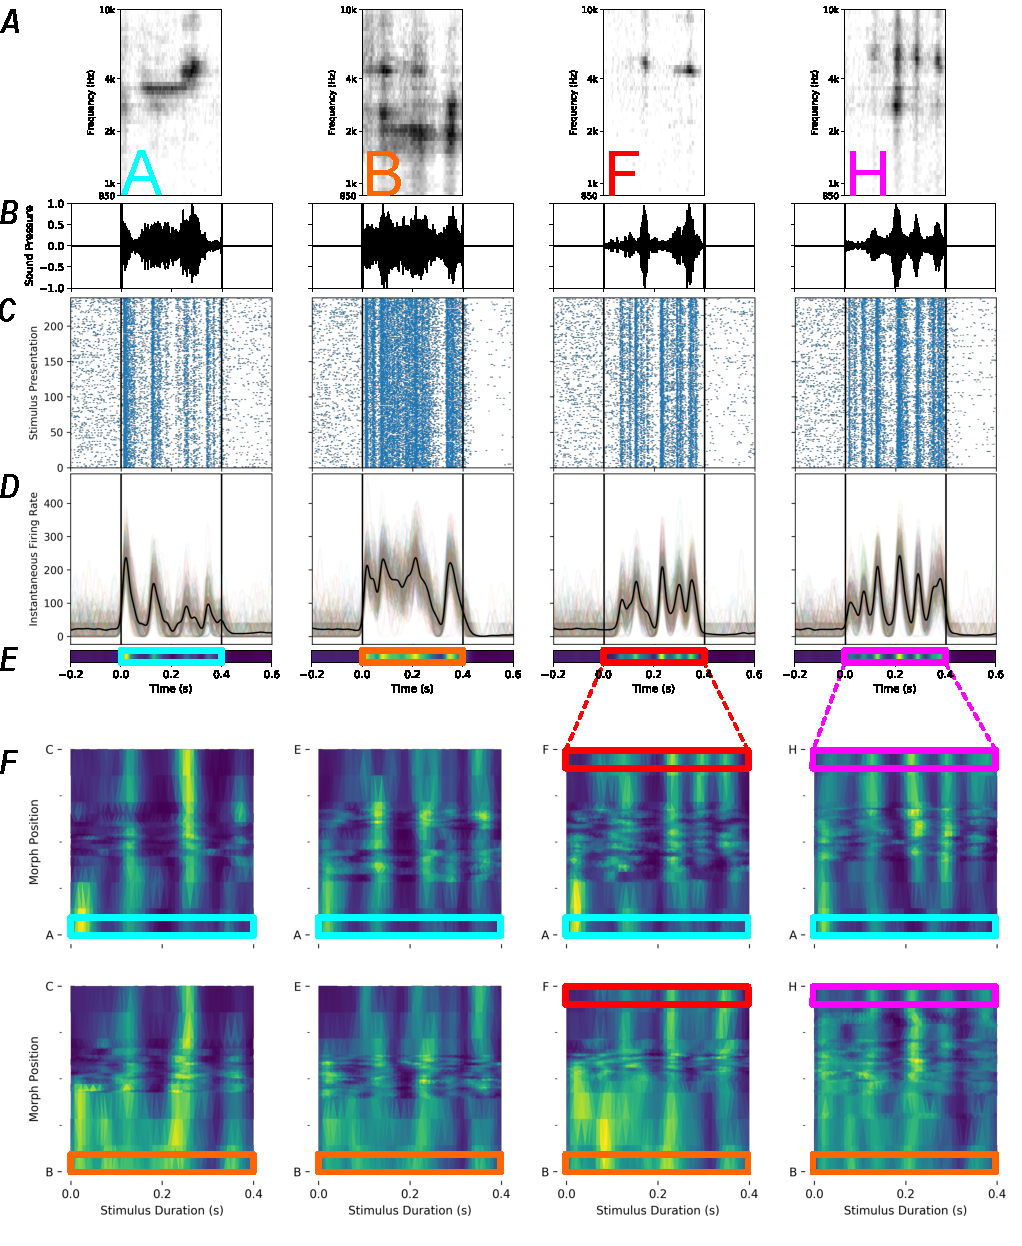
\includegraphics[width=\textwidth]{figures/fig05_single.pdf}
  \caption[Single neurons have reliable temporally precise responses]
{(continued on following page.)
\index{single}}
  \label{fig:single}
\end{figure}

\begin{figure}[tp]
  \contcaption{
(A)	Spectrogram representations of example stimuli presented to the anesthetized starlings of four example motifs presented, motifs A, B, F, and H.
(B) The equivalent audio waveform pressure representations. Black lines mark the start and end of the auditory stimuli.
(C) The raster plots of a single neuron for 240 presentations of each of these stimuli. Vertical marks are plotted at each time point of the occurrence of a spike in the 400 ms stimuli. The y-axis denotes the stimuli presentation. Black lines mark the start and end of the auditory stimuli.
(D) Average Gaussian convolved spike train representation in black. We convolve each individual trial with a Gaussian with $\sigma=10ms$ to get an instantaneous estimate of spike firing rate. These are plotted faintly to demonstrate trial to trial reliability and variance of this representation. The average of these 240 faint lines is plotted in black for each of these stimuli.
(E) Heatmap representation of the above representation to be used below. Lighter represents higher estimated instantaneous firing rate. These plots are all normalized to the max firing rate. The colored outlines indicate where the data is repeated below.
(F) Variation of the average Gaussian convolved single neuron’s representation across morph dimensions. Smoothly interpolated using triangulation for surface estimation. Morph position is plotted on the Y axis as the motif presented goes from motif A (highlighted in blue as a band along the bottom) to C (along the top) for example in the top left subplot. Time (during the stimuli presentation) is plotted on the X-axis. The representations of motif F (red) and motif H (Magenta) are diagrammed to demonstrate how the representation is using the average response of this neuron as the top row in the right two subplots in the top row of this representation. Other colors outline other areas that include the averaged representations from figure E.  Not all morph positions were presented the same number of times so confidence (not represented) varies along morph position axis.
}
\end{figure}